% want your title page.
% OR
% 2) Remove everything outside the \begin{titlepage} and \end{titlepage} and 
% move this file to the same directory as the LaTeX file you wish to add it to. 
% Then add \input{./title_page_1.tex} to your LaTeX file where you want your
% title page.
%
%%%%%%%%%%%%%%%%%%%%%%%%%%%%%%%%%%%%%%%%%
%\title{Title page with logo}
%----------------------------------------------------------------------------------------
%	PACKAGES AND OTHER DOCUMENT CONFIGURATIONS
%----------------------------------------------------------------------------------------

\documentclass[12pt]{article}
\usepackage[english]{babel}
\usepackage[utf8x]{inputenc}
\usepackage{amsmath}
\usepackage{graphicx}
\usepackage[colorinlistoftodos]{todonotes}
\usepackage{listings}
\usepackage{caption}
\usepackage{parskip} %dannati indent


\captionsetup[lstlisting]{singlelinecheck=false, margin=0pt, font={bf,footnotesize} }
\renewcommand\lstlistingname{}
\lstset{escapeinside={<@}{@>}}
\definecolor{comment}{RGB}{237, 141, 33}
\definecolor{backy}{RGB}{ 255, 253, 183 }
\definecolor{back}{RGB}{ 30,30,30 }
\definecolor{shadecolor}{RGB}{ 30,30,30 }
\definecolor{purple}{RGB}{155, 40, 140}
\lstset{
%rulecolor=\color{white},
numbers=left,
numberstyle=\color{black},
%backgroundcolor=\color{back},   
frame=single,
showspaces=false,
basicstyle=\ttfamily,%\color{white},
showstringspaces=false,
keywordstyle=\color{purple},       % keyword style
commentstyle=\color{comment},    % comment style
stringstyle=\color{blue}    % string literal style
}




\begin{document}

\begin{titlepage}

\newcommand{\HRule}{\rule{\linewidth}{0.5mm}} % Defines a new command for the horizontal lines, change thickness here

\center % Center everything on the page
 
%----------------------------------------------------------------------------------------
%	HEADING SECTIONS
%----------------------------------------------------------------------------------------

\textsc{\LARGE Università di Bergamo}\\[1.5cm] % Name of your university/college
\textsc{\Large Relazione progetto}\\[0.5cm] % Major heading such as course name
\textsc{\large Linguaggi Formali e Compilatori}\\[0.5cm] % Minor heading such as course title

%----------------------------------------------------------------------------------------
%	TITLE SECTION
%----------------------------------------------------------------------------------------

\HRule \\[0.4cm]
{ \huge \bfseries Parser ISA Risc-V}\\[0.4cm] % Title of your document
\HRule \\[1.5cm]
 
%----------------------------------------------------------------------------------------
%	AUTHOR SECTION
%----------------------------------------------------------------------------------------

\begin{minipage}{0.4\textwidth}
\begin{flushleft} \large
\emph{Autore:}\\
Dario \textsc{Sardi} % Your name
\end{flushleft}
\end{minipage}
~
\begin{minipage}{0.4\textwidth}
\begin{flushright} \large
\emph{Supervisore:} \\
Giuseppe \textsc{Psaila} % Supervisor's Name
\end{flushright}
\end{minipage}\\[2cm]

% If you don't want a supervisor, uncomment the two lines below and remove the section above
%\Large \emph{Author:}\\
%John \textsc{Smith}\\[3cm] % Your name

%----------------------------------------------------------------------------------------
%	DATE SECTION
%----------------------------------------------------------------------------------------

{\large 12 Marzo 2019}\\[2cm] % Date, change the \today to a set date if you want to be precise

%----------------------------------------------------------------------------------------
%	LOGO SECTION
%----------------------------------------------------------------------------------------


\includegraphics[scale=0.5]{logo.png}\\[1cm] % Include a department/university logo - this will require the graphicx package
 
%----------------------------------------------------------------------------------------

\vfill % Fill the rest of the page with whitespace

\end{titlepage}


\begin{abstract}
Il progetto è volto allo sviluppo di un traduttore di un subset di istruzioni appartenenti all'ISA RISC-V da linguaggio assembly a linguaggio naturale.
\end{abstract}
\section{Output e Input}
Il programma prende come input il testo contenuto nel file "resources/input.file" e restituisce la traduzione in linguaggio naturale come output su terminale seguito da una eventuale lista di errori.
\\Un esempio di output privo di errori:
\begin{lstlisting}
    <@\textcolor{purple}{----- PARSING STARTED-------}@>
created ADDI between 1 and 12 to be saved at 10
created OR between 12 and 2 to be saved at 5
added label li
created ADD between 7 and 5 to be saved at 22
created AND between 7 and 5 to be saved at 23
label check for li
jump to line 3 if condition is true
created OR between 22 and 23 to be saved at 24
<@\textcolor{purple}{----- PARSING DONE -------}@>
\end{lstlisting}
In caso di errori l'output è il seguente:
\begin{lstlisting}
    <@\textcolor{purple}{----- PARSING STARTED-------}@>
created ADDI between 1 and 12 to be saved at 10
created OR between 12 and 2 to be saved at 5
added label li
created ADD between 7 and 5 to be saved at 22
created AND between 7 and 45 to be saved at 23

#############################
#  ERROR! PARSING STOPPED!  #
#############################
<@\textcolor{red}{ERRORS:}@>
1. label 'li' at line 4 already exist, ignoring it.
2. Lexer error at [6:15].Max register value is 30!
\end{lstlisting}






%%%%%%%%%%%%%%%%%%%%%%%%%%%%%%%%%%%%%%%%%%%%%%%%%%%%%%%%%%%%%%%%%%%%%
\section{Registri e immediati}
Per le specifiche scelte per questo progetto si prevede l'esistenza di 30 registri indirizzabili attraverso la sequenza '0xNumeroDiRegistro' dove il numero del registro è un numero intero compreso fra 0 e 30.
\\La scelta del prefisso è stata dettata dalla necessità di distinguere numeri interi e numeri dei registri durante il parsing e rendere il meno confusionario possibile il codice.
\\Per quanto riguarda gli immediati è stata prevista la dimensione massima di una word su ISA RISC-V equivalente al valore decimale 4096.
%%%%%%%%%%%%%%%%%%%%%%%%%%%%%%%%%%%%%%%%%%%%%%%%%%%%%%%%%%%%%%%%%%%%%
\section{Variabili}
È previsto l'utilizzo di variabili statiche per etichettare registri o valori notevoli.
La sintassi per dichiarare il nome di un registro è:
\begin{lstlisting}[numbers=none]
    <@\textcolor{purple}{DR}@> <@\textcolor{orange}{etichetta}@> <@\textcolor{blue}{0xNumeroDiRegistro}@>
\end{lstlisting}
Una definizione valida puo dunque essere
\begin{lstlisting}[numbers=none]
    <@\textcolor{purple}{DR}@> <@\textcolor{orange}{RegistroA}@> <@\textcolor{blue}{0x9}@>
\end{lstlisting}
Si ricorda il valore massimo assegnabile a un registro pari a 0x30 per specifiche precedentemente definite.
Per quanto riguarda le variabili, si possono creare variabili numeriche statiche di tipo Byte e Word.
Risulta possibile riservare una variabile senza inizializzarla attraverso il comando RESB per riservare un Byte  e RESW per riservare una Word.
Esempio di variabili riservate sono
\begin{lstlisting}[numbers=none]
    <@\textcolor{purple}{RESW}@> <@\textcolor{orange}{valoreMassimo}@>
    <@\textcolor{purple}{RESB}@> <@\textcolor{orange}{threshold}@>
\end{lstlisting}
Questa operazione è stata introdotta per una implementazione futura dove variabili dinamiche potranno essere assegnate o variate utilizzandole come destinazione all'interno di funzioni.
Il comando attualmente utile risulta essere la dichiarazione di una variabile con relativa inizializzazione effettuabile tramite
\begin{lstlisting}[numbers=none]
    <@\textcolor{purple}{DW}@> <@\textcolor{orange}{valoreMassimo}@> <@\textcolor{blue}{3623}@>
    <@\textcolor{purple}{DB}@> <@\textcolor{orange}{threshold}@> <@\textcolor{blue}{90}@>
\end{lstlisting}


\subsection{Error handling}
Nel caso di una dichiarazione di variabile troppo grande il programma risponderà settando la variabile a 0 e proseguendo normalmente.
\\Esempi di input-output possibili sono
\begin{lstlisting}[caption=input]
    <@\textcolor{purple}{DW}@> <@\textcolor{orange}{ciao}@> <@\textcolor{blue}{5400}@>
\end{lstlisting}
\begin{lstlisting}[caption=output]
   <@\textcolor{purple}{----- PARSING STARTED-------}@>
    defined new Word-type variable with value 0 
    named <@\textcolor{orange}{ciao}@>
   <@\textcolor{purple}{----- PARSING DONE -------}@>
   <@\textcolor{red}{ERRORS:}@>
   1.	variable value is not Word type
        (max value 4096), <@\textcolor{orange}{ciao}@> set to 0
\end{lstlisting}
Oppure 
\begin{lstlisting}[caption=input]
    <@\textcolor{purple}{DB}@> <@\textcolor{orange}{ciao}@> <@\textcolor{blue}{300}@>
\end{lstlisting}
\begin{lstlisting}[caption=output]
   <@\textcolor{purple}{----- PARSING STARTED-------}@>
    defined new Byte-type variable with value 0 
    named <@\textcolor{orange}{ciao}@>
   <@\textcolor{purple}{----- PARSING DONE -------}@>
   <@\textcolor{red}{ERRORS:}@>
   1.	variable value is not Byte type
        (max value 256), <@\textcolor{orange}{ciao}@> set to 0
\end{lstlisting}
\newpage
Altro errore può verificarsi nella dichiarazione di un registro dal numero superiore al 30

\begin{lstlisting}[caption=input]
    <@\textcolor{purple}{DR}@> <@\textcolor{orange}{reg1}@> <@\textcolor{blue}{0x50}@>
\end{lstlisting}

\begin{lstlisting}[caption=output]
    <@\textcolor{purple}{----- PARSING STARTED-------}@>
    variable <@\textcolor{orange}{reg}@> too big for register-type, set to 0
    <@\textcolor{purple}{----- PARSING DONE -------}@>
    <@\textcolor{red}{ERRORS:}@>
    1.	Lexer error at [1:9].Max register 
        value is 30!
\end{lstlisting}

Nel caso di un assegnamento ad una variabile registro un valore immediato, l'errore viene considerato grave e il parsing interrotto.



%%%%%%%%%%%%%%%%%%%%%%%%%%%%%%%%%%%%%%%%%%%%%%%%%%%%%%%%%%%%%%%%%%%%%
\newpage
\section{Le funzioni}
Il subset di istruzioni considerato prevede due tipologie di funzioni, le R-type e le I-type.
\begin{figure}[h]
    \centering
    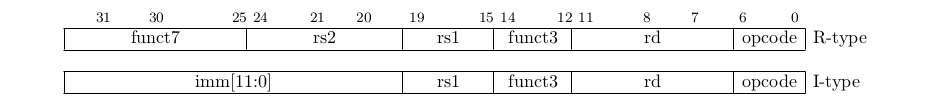
\includegraphics[scale=0.5]{functionTypes.png}
    \caption{Struttura in binario delle funzioni e relativi attributi}
    \label{fig:err1}
\end{figure}
\\
In entrambe le funzioni la struttura sintattica risulta essere
\begin{lstlisting}[numbers=none]
    <@\textcolor{purple}{Funzione}@> <@\textcolor{blue}{Destinazione Operando1 Operando2}@>
\end{lstlisting}
Per le funzioni R-type destinazione e operandi saranno registri
\begin{lstlisting}[numbers=none]
    <@\textcolor{purple}{Funzione}@> <@\textcolor{blue}{RegDestinazione RegOperando1 RegOperando2}@>
\end{lstlisting}
Per le funzioni di I-type il secondo operando dovrà essere un immediato
\begin{lstlisting}[numbers=none]
    <@\textcolor{purple}{Funzione}@> <@\textcolor{blue}{RegDestinazione RegOperando1}@> <@\textcolor{orange}{ImmOperando2}@>
\end{lstlisting}

Le funzioni previste sono le seguenti: 
\begin{enumerate}
    \item \textcolor{purple}{R-Type: ADD,SUB,MUL,OR,XOR,AND}
    \item \textcolor{purple}{I-Type: ADDI,SUBI,ORI,XORI,ANDI}
\end{enumerate}
Esempi di funzioni sono 
\begin{lstlisting}[caption=input]
    <@\textcolor{purple}{ADDI}@> <@\textcolor{blue}{0x10 0x01}@> <@\textcolor{orange}{12}@>
    <@\textcolor{purple}{OR}@> <@\textcolor{blue}{0x05 0x12 0x02}@>
\end{lstlisting}
\begin{lstlisting}[caption=output]
    <@\textcolor{purple}{ ----- PARSING STARTED------- }@>
    created ADDI between 1 and 12 to be saved at 10
    created OR between 12 and 2 to be saved at 5
    <@\textcolor{purple}{ ----- PARSING DONE------- }@>
\end{lstlisting}
\subsection{Error Handling}
Gli unici errori possibili in una funzione sono l'utilizzo di numeri di registri errati,di variabili errate (registro al posto di immediato e viceversa) o immediati di dimensione superiore alla word.
\\Nel caso di registri troppo grandi l'errore è trasmesso direttamente dal controllo su ogni singolo valore di registro e causa l'interruzione del parsing.
\begin{lstlisting}[caption=input]
    <@\textcolor{purple}{DR}@> <@\textcolor{orange}{reg}@> <@\textcolor{blue}{0x10}@>
    <@\textcolor{purple}{ADD}@> <@\textcolor{orange}{reg reg}@> <@\textcolor{blue}{0x50}@> 
\end{lstlisting}

\begin{lstlisting}[caption=output]
    <@\textcolor{purple}{ ----- PARSING STARTED------- }@>
    defined new Register variable with value 
     10 named <@\textcolor{orange}{reg}@> 

    #############################
    #  ERROR! PARSING STOPPED!  #
    #############################
    <@\textcolor{red}{ERRORS:}@>
    1.	Lexer error at [2:14].Max register value 
        is 30!
\end{lstlisting}
\newpage
L'utilizzo di variabili errate è contemplato e causa l'interruzione del parsing:
\begin{lstlisting}[caption=input]
    <@\textcolor{purple}{DR}@> <@\textcolor{orange}{reg}@> <@\textcolor{blue}{0x10}@>
    <@\textcolor{purple}{DW}@> <@\textcolor{orange}{c}@> <@\textcolor{blue}{12}@>
    <@\textcolor{purple}{ADD}@> <@\textcolor{orange}{reg reg c}@> 
\end{lstlisting}
\begin{lstlisting}[caption=output]
    <@\textcolor{purple}{ ----- PARSING STARTED------- }@>
    defined new Register variable with value 
     10 named <@\textcolor{orange}{reg}@> 
    defined new Word-type variable with value 
     12 named <@\textcolor{orange}{c}@>
    
    #############################
    #  ERROR! PARSING STOPPED!  #
    #############################
    <@\textcolor{red}{ERRORS:}@>
    1.	at line 3 using a non register variable
\end{lstlisting}


%%%%%%%%%%%%%%%%%%%%%%%%%%%%%%%%%%%%%%%%%%%%%%%%%%%%%%%%%%%%%%%%%%%%%
\section{Loop}


\subsection{Error Handling}


%%%%%%%%%%%%%%%%%%%%%%%%%%%%%%%%%%%%%%%%%%%%%%%%%%%%%%%%%%%%%%%%%%%%%
\end{document}